\documentclass[12pt,a4paper]{report}

% =========================================================
% 1. PACKAGES FONDAMENTAUX & TYPOGRAPHIE
% =========================================================
\usepackage[T1]{fontenc}
\usepackage[utf8]{inputenc}
\usepackage[french]{babel}
\usepackage{lmodern}
\usepackage{microtype}
\usepackage{setspace}
\onehalfspacing

% Marges standard
\usepackage{geometry}
\geometry{
    top=2.5cm,
    bottom=2.5cm,
    left=3cm,
    right=2.5cm
}

% =========================================================
% 2. GRAPHIQUES & TABLEAUX
% =========================================================
\usepackage{graphicx}
\graphicspath{{Images/}{images/}}
\usepackage{pdfpages}
\usepackage{float}
\usepackage{booktabs}
\usepackage{array}
\usepackage{tabularx}
\usepackage[table]{xcolor}
\usepackage{amsmath,amssymb}
\usepackage{textcomp}

% =========================================================
% 3. EN-TÊTES ET PIEDS DE PAGE (TOUT EN NOIR)
% =========================================================
\usepackage{fancyhdr}
\pagestyle{fancy}
\fancyhf{}
\fancyhead[L]{\small\nouppercase{\leftmark}}
\fancyhead[R]{\small PFE - Smart Fiber}
\fancyfoot[C]{\thepage}
\renewcommand{\headrulewidth}{0.4pt}
\renewcommand{\footrulewidth}{0.0pt}

\fancypagestyle{plain}{
    \fancyhf{}
    \fancyfoot[C]{\thepage}
    \renewcommand{\headrulewidth}{0pt}
}

% =========================================================
% 4. FORMATTAGE DES TITRES (TOUS EN NOIR)
% =========================================================
\usepackage{titlesec}
\titleformat{\chapter}[display]
  {\normalfont\huge\bfseries\color{black}}
  {\chaptertitlename\ \thechapter}{15pt}{\Huge\color{black}}
\titlespacing*{\chapter}{0pt}{10pt}{25pt}

\titleformat{\section}
  {\normalfont\Large\bfseries\color{black}}{\thesection}{1em}{}

\titleformat{\subsection}
  {\normalfont\large\bfseries\color{black}}{\thesubsection}{1em}{}

\titleformat{\subsubsection}
  {\normalfont\normalsize\bfseries\color{black}}{\thesubsubsection}{1em}{}

% =========================================================
% 5. HYPERLIENS & MÉTADONNÉES PDF (TEXTE DES LIENS EN NOIR)
% =========================================================
\usepackage{hyperref}
\hypersetup{
    colorlinks=true,
    linkcolor=black,
    citecolor=black,
    urlcolor=black,
    pdftitle={Rapport de Projet de Fin d'Etudes - Smart Fiber Supervision},
    pdfauthor={Ben Zineb Amir},
    pdfsubject={Diplôme National d'Ingénieur en Informatique}
}

% =========================================================
% DÉBUT DU DOCUMENT
% =========================================================
\begin{document}

% ---------------------------------------------------------
% PAGE DE GARDE & VALIDATION
% ---------------------------------------------------------

\includepdf[pages=-]{PageG2.pdf}

% ---------------------------------------------------------
% PARTIE PRÉLIMINAIRE (Numérotation romaine)
% ---------------------------------------------------------
\pagenumbering{roman}
\setcounter{page}{1}

\chapter*{Remerciements}
\addcontentsline{toc}{chapter}{Remerciements}

Au terme de ce projet de fin d'études, réalisé au sein de \textbf{Tunisie Telecom} pour l'obtention du Diplôme National d'Ingénieur en Informatique à l'\textbf{École Supérieure Privée d'Ingénierie et de Technologies (ESPRIT)}, je tiens à exprimer ma profonde gratitude et mes sincères remerciements à toutes les personnes qui ont contribué à la réussite de ce travail.

Je tiens tout d'abord à remercier chaleureusement mon encadrant professionnel chez \textbf{Tunisie Telecom}, pour son accueil, sa confiance, ses orientations précieuses et son soutien continu tout au long de cette expérience enrichissante.

J'adresse également mes vifs remerciements à mon encadrant académique à \textbf{ESPRIT}, pour sa disponibilité, ses conseils méthodologiques avisés et son suivi rigoureux qui m'ont permis de mener à bien ce projet dans les meilleures conditions.

Mes sincères remerciements vont également à l'ensemble du corps professoral et administratif d'ESPRIT pour la qualité de la formation dispensée durant mon cursus d'ingénieur.

Enfin, j'exprime ma gratitude envers les honorables membres du jury qui nous font l'honneur d'évaluer ce travail. Que chacun trouve ici le témoignage de mon profond respect.

\chapter*{R\'esum\'es}
\addcontentsline{toc}{chapter}{R\'esum\'es}

\subsection*{R\'esum\'e}
Dans un contexte d'expansion acc\'el\'er\'ee des r\'eseaux de t\'el\'ecommunications \`a tr\`es haut d\'ebit, l'exploitation et la maintenance proactive des infrastructures de fibre optique (FTTH) constituent un enjeu strat\'egique majeur pour les op\'erateurs. Ce projet de fin d'\'etudes, men\'e au sein de \textbf{Tunisie Telecom}, vise \`a concevoir et d\'evelopper une plateforme logicielle int\'egr\'ee de supervision r\'eseau et d'aide \`a la d\'ecision. 

La solution r\'ealis\'ee s'articule autour d'une architecture client-serveur modulaire et d\'ecoupl\'ee, compos\'ee d'une application mobile moderne d\'evelopp\'ee avec \textbf{Flutter} et d'une API back-end haute performance propuls\'ee par \textbf{NestJS}. Elle combine une cartographie g\'eographique interactive multi-couches (NRO, FDT, clients et c\^ablages), une diffusion d'\'ev\'enements et d'alertes en temps r\'eel via \textbf{WebSockets (Socket.IO)}, ainsi que des modules avanc\'es d'\textbf{intelligence artificielle} (int\'egration Groq LLM avec m\'ecanisme de r\'esilience Circuit Breaker et heuristiques m\'etier) pour la qualification automatis\'ee des r\'eclamations abonn\'es et l'anticipation de la saturation des n\oe uds de raccordement optique. Le projet a \'et\'e men\'e selon la m\'ethodologie \textbf{Agile Scrum}, aboutissant \`a une solution robuste, scalable et ergonomique pour les \'equipes techniques et op\'erationnelles.

\vspace{0.3cm}
\textbf{Mots-cl\'es :} Supervision T\'el\'ecom, Fibre Optique (FTTH), NRO, FDT, Flutter, NestJS, Socket.IO, SIG / Cartographie, Intelligence Artificielle, Circuit Breaker, Scrum.

\vspace{0.8cm}
\subsection*{Abstract}
In the context of the rapid expansion of high-speed telecommunication networks, proactive operation and maintenance of optical fiber infrastructures (FTTH) represent a critical strategic challenge for telecom operators. This graduation project, conducted at \textbf{Tunisie Telecom}, aims to design and implement an integrated network supervision and decision-support platform.

The developed solution is based on a decoupled, modular client-server architecture, featuring a cross-platform mobile application built with \textbf{Flutter} and a scalable backend API powered by \textbf{NestJS}. The platform integrates interactive multi-layer GIS mapping (NRO, FDT, clients, and fiber cables), real-time event and alert streaming via \textbf{WebSockets (Socket.IO)}, and advanced \textbf{Artificial Intelligence} modules (Groq LLM inference with a resilient Circuit Breaker mechanism and domain heuristics) for automated ticket classification and optical node saturation forecasting. Developed using the \textbf{Agile Scrum} framework, the resulting solution provides a robust, real-time, and user-friendly monitoring tool for field technicians and network administrators.

\textbf{Keywords:} Telecom Supervision, Optical Fiber, FTTH, NRO, FDT, Flutter, NestJS, Socket.IO, GIS Mapping, Artificial Intelligence, Circuit Breaker, Agile Scrum.


\tableofcontents
\newpage

\listoffigures
\newpage

\listoftables
\newpage

\chapter*{Liste des abr\'eviations}
\addcontentsline{toc}{chapter}{Liste des abr\'eviations}

\begin{table}[H]
\centering
\begin{tabularx}{\textwidth}{lX}
\toprule
\textbf{Abr\'eviation} & \textbf{Signification} \\
\midrule
\textbf{API}   & Application Programming Interface \\
\textbf{CI/CD} & Continuous Integration / Continuous Deployment \\
\textbf{CRUD}  & Create, Read, Update, Delete \\
\textbf{DTO}   & Data Transfer Object \\
\textbf{FDT}   & Fiber Distribution Terminal (Sous-r\'epartiteur optique) \\
\textbf{FTTH}  & Fiber To The Home \\
\textbf{GIS / SIG} & Syst\`eme d'Information G\'eographique \\
\textbf{GPON}  & Gigabit Passive Optical Network \\
\textbf{HTTP}  & HyperText Transfer Protocol \\
\textbf{JSON}  & JavaScript Object Notation \\
\textbf{JWT}   & JSON Web Token \\
\textbf{KPI}   & Key Performance Indicator \\
\textbf{LLM}   & Large Language Model \\
\textbf{NLP}   & Natural Language Processing \\
\textbf{NRO}   & N\oe ud de Raccordement Optique \\
\textbf{ODM}   & Object Data Modeling \\
\textbf{OLT}   & Optical Line Terminal \\
\textbf{ONT}   & Optical Network Terminal \\
\textbf{QA}    & Quality Assurance \\
\textbf{RBAC}  & Role-Based Access Control \\
\textbf{REST}  & Representational State Transfer \\
\textbf{UML}   & Unified Modeling Language \\
\textbf{URI}   & Uniform Resource Identifier \\
\textbf{WS}    & WebSocket \\
\bottomrule
\end{tabularx}
\end{table}

\newpage

% ---------------------------------------------------------
% CORPS DU RAPPORT (Numérotation arabe : 1, 2, 3...)
% Structure exacte correspondant à votre rapport de 89 pages
% ---------------------------------------------------------
\pagenumbering{arabic}
\setcounter{page}{1}

\chapter*{Introduction g\'en\'erale}
\addcontentsline{toc}{chapter}{Introduction g\'en\'erale}

\section*{Contexte g\'en\'eral}
Le secteur des t\'el\'ecommunications conna\^it une transformation num\'erique sans pr\'ec\'edent, marqu\'ee par le d\'eploiement massif des r\'eseaux d'acc\`es \`a tr\`es haut d\'ebit en fibre optique jusqu'\`a l'abonn\'e (\textit{Fiber To The Home} - FTTH). Les op\'erateurs t\'el\'ecoms doivent g\'erer des infrastructures optiques complexes compos\'ees de milliers d'\'el\'ements physiques interconnect\'es : N\oe uds de Raccordement Optique (NRO), Sous-r\'epartition Optique (FDT), c\^ables de transport et de distribution, et points de branchement abonn\'es.

Dans cet \'ecosyst\`eme hautement dynamique, la qualit\'e de service (QoS) et l'exp\'erience utilisateur (QoE) reposent sur la capacit\'e \`a d\'etecter, localiser et r\'esoudre les incidents r\'eseau dans les plus brefs d\'elais, tout en pr\'evenant la saturation des \'equipements.

\section*{Probl\'ematique}
Au sein de l'op\'erateur national \textbf{Tunisie Telecom}, la supervision et la gestion des interventions reposaient traditionnellement sur des outils partiellement h\'et\'erog\`enes et cloisonn\'es. Les \'equipes d'exploitation et les techniciens d'intervention terrain faisaient face \`a plusieurs contraintes critiques :
\begin{itemize}
    \item \textbf{Absence de vue cartographique unifi\'ee en temps r\'eel :} Difficult\'e \`a visualiser simultan\'ement sur une m\^eme carte g\'eographique l'\'etat op\'erationnel des NRO, des FDT et des contrats clients rattach\'es.
    \item \textbf{Latence dans le traitement des \'ev\'enements :} Manque d'un canal de communication bidirectionnel instantan\'e pour notifier les \'equipes des alertes et changements d'\'etat sans rechargement manuel.
    \item \textbf{Qualification manuelle des r\'eclamations :} Volume important de r\'eclamations d'abonn\'es n\'ecessitant un tri et une affectation manuels souvent chronophages.
    \item \textbf{Difficult\'e d'anticipation de la saturation :} Absence d'indicateurs pr\'edictifs automatis\'es pour alerter sur le taux de remplissage critique des ports et des capacit\'es d'un NRO avant blocage.
\end{itemize}

Face \`a ce constat, la probl\'ematique centrale de ce projet de fin d'\'etudes s'articule autour de la question suivante : \textit{Comment concevoir et d\'evelopper une plateforme logicielle moderne, r\'eactive et intellignete, capable de centraliser la supervision cartographique du r\'eseau fibre, de traiter les \'ev\'enements en temps r\'eel et d'apporter une aide \`a la d\'ecision gr\^ace \`a l'intelligence artificielle ?}

\section*{Objectifs du projet}
Pour r\'epondre \`a ces d\'efis, notre mission a consist\'e \`a concevoir et d\'evelopper une solution compl\`ete comprenant :
\begin{enumerate}
    \item Une \textbf{application mobile multiplateforme en Flutter}, offrant une interface ergonomique adapt\'ee aux techniciens terrain et aux superviseurs r\'egionaux, avec navigation par r\^oles (RBAC) et cartographie interactive multi-couches.
    \item Un \textbf{back-end modulaire et scalable en NestJS (TypeScript)}, exposant des API REST s\'ecuris\'ees, une passerelle WebSocket pour le temps r\'eel (Socket.IO), et une file de traitement asynchrone (BullMQ/Redis).
    \item Un \textbf{moteur d'intelligence m\'etier (IA)} int\'egrant l'inf\'erence LLM haute vitesse via Groq, renforc\'e par un disjoncteur (\textit{Circuit Breaker}) et des mod\`eles heuristiques pour la classification des tickets et la d\'etection pr\'eventive de la saturation NRO.
\end{enumerate}

\section*{D\'emarche m\'ethodologique}
Afin d'assurer une r\'eactivit\'e face aux \'evolutions du besoin et une livraison incr\'ementale de valeur, nous avons adopt\'e la d\'emarche \textbf{Agile Scrum}. Le projet a \'et\'e structur\'e en 3 grandes Releases r\'eparties sur 12 it\'erations (Sprints S0 \`a S11), favorisant une int\'egration continue des retours m\'etier.

\section*{Structure du rapport}
Le pr\'esent rapport retrace les diff\'erentes phases du projet et s'organise en cinq chapitres principaux :
\begin{itemize}
    \item \textbf{Chapitre 1 -- Contexte du projet et \'Etat de l'art :} pr\'esente l'organisme d'accueil Tunisie Telecom, l'\'etude de l'existant, la probl\'ematique m\'etier, la justification des choix m\'ethodologiques et architecturaux, ainsi que l'\'etat de l'art des technologies retenues.
    \item \textbf{Chapitre 2 -- Analyse des besoins et conception g\'en\'erale :} d\'efinit les exigences fonctionnelles et non fonctionnelles, formalise les cas d'utilisation globaux et expose le mod\`ele de donn\'ees conceptuel du syst\`eme.
    \item \textbf{Chapitre 3 -- Release 1 : Socle technique, Authentification et Gestion des Utilisateurs :} d\'etaille la mise en place de l'architecture, la s\'ecurit\'e JWT/RBAC et la r\'ealisation des interfaces d'administration des comptes.
    \item \textbf{Chapitre 4 -- Release 2 : Supervision r\'eseau, Cartographie et Temps r\'eel :} expose la mise en \oe uvre de la cartographie interactive multi-couches, du protocole de diffusion temps r\'eel et des tableaux de bord KPI.
    \item \textbf{Chapitre 5 -- Release 3 : IA m\'etier, Tests, D\'eploiement et Industrialisation :} pr\'esente l'int\'egration des modules d'intelligence artificielle (Groq LLM \& saturation NRO), la strat\'egie de tests logiciels, le diagramme de d\'eploiement et l'infrastructure de production.
\end{itemize}
Le rapport se cl\^oture par une \textbf{Conclusion g\'en\'erale} qui dresse le bilan des r\'ealisations et ouvre des perspectives d'\'evolution pour la solution.
     % Introduction générale
\chapter{Contexte du projet et \'Etat de l'art}
\label{chap:contexte}

\section*{Introduction}
Dans ce premier chapitre, nous introduisons le cadre g\'en\'eral de notre projet de fin d'\'etudes r\'ealis\'e au sein de \textbf{Tunisie Telecom}. Nous commen\c{c}ons par pr\'esenter l'organisme d'accueil, son positionnement strat\'egique et les sp\'ecificit\'es li\'ees \`a l'exploitation des r\'eseaux de fibre optique. Nous exposons ensuite l'\'etude de l'existant, la probl\'ematique m\'etier identifi\'ee et la solution globale propos\'ee. Enfin, nous justifions le choix de la m\'ethodologie de conduite de projet (Agile Scrum), le choix de l'architecture logicielle retenue (\'Ecosyst\`eme 3-Tiers d\'ecoupl\'e), ainsi qu'une revue d\'etaill\'ee des technologies front-end, back-end et d'infrastructure adopt\'ees.

\section{Pr\'esentation de l'entreprise d'accueil}
Le projet a \'et\'e r\'ealis\'e au sein de \textbf{Tunisie Telecom}, l'op\'erateur historique et leader des t\'el\'ecommunications en Tunisie. Fond\'e pour offrir des services t\'el\'ecoms int\'egr\'es (fixe, mobile, transmission de donn\'ees et acc\`es Internet tr\`es haut d\'ebit), l'op\'erateur dessert plusieurs millions d'abonn\'es r\'esidentiels et professionnels \`a travers tout le territoire tunisien.

\begin{figure}[H]
 \centering
 
\includegraphics[width=6cm]{Images/LOGO_TT_.png}
 \caption{Logo officiel de Tunisie Telecom}
 \label{fig:logo_tt}
\end{figure}

Dans le cadre du d\'eploiement massif de son r\'eseau \textbf{FTTH (Fiber To The Home)}, Tunisie Telecom g\`ere une infrastructure optique passive et active d'envergure nationale, articul\'ee autour de composants cl\'es :
\begin{itemize}
    \item \textbf{Le NRO (N\oe ud de Raccordement Optique) :} C\oe ur du r\'eseau local abritant les \'equipements actifs (OLT -- Optical Line Terminal) et assurant la distribution de la capacit\'e optique vers les diff\'erentes zones g\'eographiques.
    \item \textbf{Le FDT (Fiber Distribution Terminal) :} Sous-r\'epartiteur optique interm\'ediaire o\`u les c\^ables de transport sont divis\'es en c\^ables de distribution vers les points de mutualisation et de branchement.
    \item \textbf{Les contrats abonn\'es et raccordements :} Points terminaux reliant les clients finaux (ONT) aux infrastructures d'acc\`es.
\end{itemize}

Face \`a cette densification r\'eseau, la disponibilit\'e d'outils num\'eriques de cartographie dynamique, de supervision en temps r\'eel et d'aide automatis\'ee \`a la d\'ecision est devenue un imp\'eratif pour maintenir l'excellence op\'erationnelle.

\section{Mission et objectifs du projet}
La mission confi\'ee consiste \`a concevoir, d\'evelopper et d\'eployer une plateforme de supervision intelligente orient\'ee m\'etier, articul\'ee autour de deux composantes logicielles majeures :
\begin{itemize}
    \item Un \textbf{front-end mobile (Flutter)} d\'edi\'e aux techniciens terrain et aux responsables r\'egionaux ;
    \item Une \textbf{API back-end (NestJS)} robuste centralisant la s\'ecurit\'e, le traitement des flux d'\'ev\'enements, la gestion cartographique et les services d'intelligence artificielle.
\end{itemize}

Les objectifs principaux du projet sont :
\begin{itemize}
    \item Assurer une \textbf{gouvernance stricte des acc\`es} bas\'ee sur les r\^oles (RBAC) et les p\'erim\`etres g\'eographiques (Zones d'affectation) ;
    \item Offrir une \textbf{cartographie interactive multi-couches} permettant de visualiser et filtrer les NRO, FDT, clients et zones g\'eographiques ;
    \item Mettre en place un \textbf{moteur temps r\'eel} pour la r\'eception instantan\'ee des \'ev\'enements m\'etier et des alertes de pannes ;
    \item Int\'egrer des \textbf{modules d'IA d'aide \`a la d\'ecision} : enrichissement et classification intelligente des r\'eclamations abonn\'es, et calcul pr\'eventif des indices de saturation des NRO.
\end{itemize}

\section{\'Etude de l'existant et limites}
Avant la mise en place de notre solution, le suivi op\'erationnel du r\'eseau reposait sur des processus semi-manuels et des outils dispers\'es. L'analyse critique de l'existant a mis en exergue plusieurs limites majeures :
\begin{itemize}
    \item \textbf{Fragmentation des sources d'information :} Manque de corr\'elation visuelle entre les incidents d\'eclar\'es et leur localisation exacte sur l'infrastructure physique.
    \item \textbf{Absence de canal temps r\'eel natif :} Les \'equipes devaient actualiser manuellement leurs interfaces pour d\'etecter les nouveaux tickets d'incident.
    \item \textbf{Processus d'escalade lent pour les r\'eclamations :} L'analyse textuelle des r\'eclamations \'etait effectu\'ee manuellement par les op\'erateurs de support, augmentant le d\'elai moyen de r\'esolution (MTTR).
    \item \textbf{Gestion r\'eactive plut\^ot que pr\'eventive de la capacit\'e :} La saturation des \'equipements optiques \'etait g\'en\'eralement d\'ecouverte lors du refus d'activation d'un nouvel abonn\'e.
\end{itemize}

\section{Probl\'ematique et solution propos\'ee}

\subsection{Probl\'ematique}
Au regard des limites constat\'ees, la probl\'ematique de recherche et de d\'eveloppement se r\'esume ainsi :
\begin{quote}
\textit{\og Comment concevoir et mettre en \oe uvre une plateforme de supervision mobile et r\'eactive, capable d'unifier la visualisation cartographique des r\'eseaux optiques FTTH, d'assurer une ingestion d'\'ev\'enements temps r\'eel et d'int\'egrer des capacit\'es d'intelligence artificielle pour optimiser l'exploitation op\'erationnelle ? \fg}
\end{quote}

\subsection{Solution propos\'ee}
Pour r\'epondre \`a cette probl\'ematique, nous proposons une architecture logicielle moderne fond\'ee sur le d\'ecouplage fonctionnel :
\begin{itemize}
    \item \textbf{Application mobile Flutter :} Une interface moderne, fluide (Material 3), offrant une cartographie enrichie (\textit{flutter\_map}), des tableaux de bord interactifs (\textit{fl\_chart}) et une gestion d'\'etat r\'eactive avec \textbf{Riverpod}.
    \item \textbf{Plateforme serveur NestJS :} Une API structur\'ee selon les principes de la \textit{Clean Architecture}, int\'egrant une s\'ecurit\'e par jetons JWT sign\'es, une persistance optimis\'ee sous \textbf{MongoDB} avec index g\'eospatiaux 2dsphere, une passerelle \textbf{Socket.IO} pour la diffusion temps r\'eel et une file de t\^aches asynchrones \textbf{BullMQ/Redis}.
    \item \textbf{Superviseur IA :} Un micro-module d'analyse s\'emantique exploitant l'inf\'erence LLM haute performance via Groq et des algorithmes d'analyse capacitaire.
\end{itemize}

\section{Choix de la m\'ethodologie de travail}

\subsection{Comparatif : Approches traditionnelles vs M\'ethodes agiles}
Le tableau~\ref{tab:metho} synth\'etise les diff\'erences entre les mod\`eles de d\'eveloppement s\'equentiels et les mod\`eles agiles.

\begin{table}[H]
\centering
\begin{tabular}{|p{3.5cm}|p{5.5cm}|p{5.5cm}|}
\hline
\textbf{Crit\`ere} & \textbf{Approches traditionnelles (Cascade/V)} & \textbf{M\'ethodes Agiles (Scrum)} \\
\hline
Cycle de d\'eveloppement & S\'equentiel, rigide et phases ferm\'ees & It\'eratif, incr\'emental et \'evolutif \\
\hline
Gestion du changement & Co\^uteuse, difficile et tardive & Continue, adaptative et flexible \\
\hline
Implication client/m\'etier & Limit\'ee aux phases initiales et finales & R\'eguli\`ere \`a chaque fin de sprint \\
\hline
Livraison & Monolithique en fin de projet & Incr\'ements fonctionnels fr\'equents \\
\hline
Traitement des risques & Risques d\'etect\'es tardivement & R\'esolution pr\'ecoce et continue \\
\hline
\end{tabular}
\caption{Comparaison entre m\'ethodologies traditionnelles et m\'ethodes agiles}
\label{tab:metho}
\end{table}

\subsection{M\'ethodologie retenue : Agile Scrum}
Compte tenu de la complexit\'e technique (cartographie mobile, int\'egrations temps r\'eel et modules IA) et du besoin de valider r\'eguli\`erement les fonctionnalit\'es aupr\`es des utilisateurs, le framework \textbf{Scrum} a \'et\'e adopt\'e. 
Le projet a \'et\'e structur\'e en 3 releases majeures compos\'ees de sprints d'une \`a deux semaines :
\begin{itemize}
    \item \textbf{Release 1 (S0 \`a S3) :} Cadrage, socle architectural, authentification et administration des utilisateurs ;
    \item \textbf{Release 2 (S4 \`a S7) :} Supervision cartographique multi-couches, temps r\'eel et tableaux de bord KPI ;
    \item \textbf{Release 3 (S8 \`a S11) :} Int\'egration de l'IA (Groq LLM \& saturation NRO), tests d'int\'egration et industrialisation.
\end{itemize}

\section{Choix architectural}

\subsection{Comparatif des styles architecturaux}
Le tableau~\ref{tab:archi} compare les principaux styles d'architecture logicielle.

\begin{table}[H]
\centering
\begin{tabular}{|p{3.2cm}|p{3.8cm}|p{3.8cm}|p{4.2cm}|}
\hline
\textbf{Crit\`ere} & \textbf{Monolithique} & \textbf{Microservices} & \textbf{Client-Serveur modulaire 3-Tiers} \\
\hline
Complexit\'e initiale & Faible & Tr\`es \'elev\'ee & Mod\'er\'ee et ma\^itris\'ee \\
\hline
D\'ecouplage & Faible & Tr\`es \'elev\'e & \'Elev\'e (Front/Back/BDD isol\'es) \\
\hline
D\'eploiement & Unique et lourd & Distribu\'e (Orchestration complexe) & Simplifi\'e et ind\'ependant \\
\hline
Scalabilit\'e & Limit\'ee & Excellente & Tr\`es bonne par couche \\
\hline
Maintenabilit\'e & D\'egrad\'ee \`a terme & Co\^uteuse en infrastructure & Optimale pour \'equipe agile \\
\hline
\end{tabular}
\caption{Comparaison des styles architecturaux}
\label{tab:archi}
\end{table}

\subsection{Architecture retenue : Client-Serveur modulaire d\'ecoupl\'e (3-Tiers)}
Nous avons retenu une \textbf{architecture 3-tiers modulaire et d\'ecoupl\'ee} :
\begin{enumerate}
    \item \textbf{Niveau Pr\'esentation (Front-end Mobile) :} Application mobile r\'ealis\'ee avec Flutter, organis\'ee selon le pattern \textit{Feature-First}. La logique d'affichage est strictement s\'epar\'ee de la logique m\'etier gr\^ace \`a \textbf{Riverpod}.
    \item \textbf{Niveau Logique M\'etier (Back-end API) :} Serveur d'applications bas\'e sur NestJS, structur\'e en modules fonctionnels isol\'es (\textit{AuthModule, UsersModule, NetworkModule, AiSupervisorModule, RealtimeModule}). Chaque module applique le principe de s\'eparation en couches :
    \begin{itemize}
        \item \textbf{Controllers :} R\'eception des requ\^etes HTTP et validation des DTOs ;
        \item \textbf{Services :} Logique m\'etier, algorithmes et r\`egles de gestion ;
        \item \textbf{Gateways :} Gestion des connexions bidirectionnelles WebSocket (Socket.IO) ;
        \item \textbf{Schemas / Models :} D\'efinition des mod\`eles ODM Mongoose.
    \end{itemize}
    \item \textbf{Niveau Donn\'ees et Persistance (Database \& Cache) :} 
    \begin{itemize}
        \item \textbf{MongoDB :} Base de donn\'ees orient\'ee documents avec support natif des index g\'eospatiaux \textit{2dsphere} ;
        \item \textbf{Redis :} Stockage en m\'emoire pour l'orchestration des files de messages avec \textbf{BullMQ}.
    \end{itemize}
\end{enumerate}

\section{\'Etat de l'art des technologies utilis\'ees}

\subsection{Technologies Front-End Mobile}

\subsubsection{Framework Mobile : Flutter / Dart}
\textbf{Flutter}~\cite{flutter2025} est le framework open-source d\'evelopp\'e par Google pour concevoir des applications compil\'ees nativement pour mobile (Android, iOS), web et desktop depuis un code source unique. Le langage \textbf{Dart} fournit un typage statique fort et une ex\'ecution tr\`es performante via compilation AOT (\textit{Ahead-Of-Time}).

\begin{figure}[H]
 \centering
 
\includegraphics[width=5cm]{Images/flutter.png}
 \caption{Framework Flutter / Dart}
 \label{fig:flutter}
\end{figure}

\subsubsection{Gestion d'\'etat : Riverpod}
\textbf{Riverpod}~\cite{riverpod2025} est une solution avanc\'ee de gestion d'\'etat r\'eactive pour Flutter. Elle garantit la s\'ecurit\'e \`a la compilation (\textit{compile-safe}), \'elimine les d\'ependances globales directes (\textit{BuildContext}), et optimise les rendus de widgets en \'evitant les reconstructions inutiles d'\'ecrans.

\begin{figure}[H]
 \centering
 
\includegraphics[width=4.5cm]{Images/riverpod.png}
 \caption{Gestion d'\'etat r\'eactive avec Riverpod}
 \label{fig:riverpod}
\end{figure}

\subsubsection{Client HTTP : Dio}
\textbf{Dio}~\cite{dio2025} est un client HTTP puissant pour Dart, supportant les intercepteurs (\textit{Interceptors}) permettant d'injecter automatiquement les tokens JWT dans les en-t\^etes de requ\^etes et de g\'erer le renouvellement automatique (\textit{Token Refresh}) en cas d'expiration.

\begin{figure}[H]
 \centering
 
\includegraphics[width=4.5cm]{Images/dio.png}
 \caption{Client r\'eseau Dio pour Flutter}
 \label{fig:dio}
\end{figure}

\subsubsection{Cartographie interactive : flutter\_map et latlong2}
La biblioth\`eque \textbf{flutter\_map}~\cite{fluttermap2025} bas\'ee sur les tuiles OpenStreetMap permet de superposer dynamiquement des couches g\'eographiques (polygones de zones de couverture, marqueurs personnalis\'es de NRO/FDT et trac\'es de liaisons optiques).

\subsection{Technologies Back-End et Persistance}

\subsubsection{Framework Back-End : NestJS / TypeScript}
\textbf{NestJS}~\cite{nestjs2025} est un framework Node.js d'entreprise fond\'e sur TypeScript. Il b\'en\'eficie d'une architecture modulaire inspir\'ee d'Angular (Injection de D\'ependances, D\'ecorateurs, Middlewares, Guards et Intercepteurs), garantissant une tr\`es grande maintenabilit\'e et testabilit\'e.

\begin{figure}[H]
 \centering
 
\includegraphics[width=4.5cm]{Images/nestjs.png}
 \caption{Framework serveur NestJS}
 \label{fig:nestjs}
\end{figure}

\subsubsection{Base de donn\'ees : MongoDB \& ODM Mongoose}
\textbf{MongoDB}~\cite{mongodb2025} est un syst\`eme de gestion de base de donn\'ees NoSQL orient\'e documents JSON/BSON. Associ\'e \`a l'ODM \textbf{Mongoose}, il permet d'exploiter des index g\'eospatiaux \textit{2dsphere} indispensables pour ex\'ecuter des requ\^etes spatiales complexes (\texttt{\$geoWithin}, \texttt{\$near}, \texttt{\$geoIntersects}).

\begin{figure}[H]
 \centering
 
\includegraphics[width=4.5cm]{Images/mongodb.png}
 \caption{Base de donn\'ees NoSQL MongoDB}
 \label{fig:mongodb}
\end{figure}

\subsubsection{Traitement asynchrone et files de t\^aches : BullMQ + Redis}
\textbf{BullMQ}~\cite{bullmq2025}, aliment\'e par \textbf{Redis}, permet d'ing\'erer des volumes \'elev\'es d'\'ev\'enements m\'etier en arri\`ere-plan sans bloquer la boucle d'\'ev\'enements principale du serveur Node.js.

\begin{figure}[H]
 \centering
 
\includegraphics[width=4.5cm]{Images/bullmq.png}
 \caption{Orchestration asynchrone BullMQ \& Redis}
 \label{fig:bullmq}
\end{figure}

\subsection{Environnement de d\'eveloppement, tests et d\'eploiement}
\begin{itemize}
    \item \textbf{Vercel / Cloud Infrastructure}~\cite{vercel2025} : Utilis\'e pour l'h\'ebergement cloud continu et la centralisation des configurations d'environnement.
    \item \textbf{Backend Mock Local} : Utilis\'e durant les phases de d\'eveloppement initial pour simuler les \'equipements t\'el\'ecoms distants et valider les sc\'enarios d'injection d'\'ev\'enements de test.
    \item \textbf{Journalisation structur\'ee (Qlog / Winston)} : Assure la tra\c{c}abilit\'e, l'audit des requ\^etes et la r\'esolution rapide des anomalies de production.
\end{itemize}

\section*{Conclusion}
Ce premier chapitre a permis d'ancrer le projet dans son contexte industriel aupr\`es de \textbf{Tunisie Telecom} et de poser les fondements m\'ethodologiques et architecturaux. Nous avons justifi\'e l'adoption d'Agile Scrum, d'une architecture client-serveur modulaire 3-tiers, et d'une suite technologique moderne (Flutter, NestJS, MongoDB, Socket.IO, BullMQ). Le chapitre suivant sera consacr\'e \`a la sp\'ecification d\'etaill\'ee des besoins et \`a la conception globale du syst\`eme.
         % Chapitre 1 : Contexte du projet et État de l'art
\chapter{Analyse des besoins et conception g\'en\'erale}
\label{chap:requirements}

\section*{Introduction}
Avant d'entamer l'impl\'ementation technique, il est primordial de d\'elimiter pr\'ecis\'ement le p\'erim\`etre fonctionnel et technique de la plateforme. Ce deuxi\`eme chapitre a pour vocation de sp\'ecifier les exigences fonctionnelles et non fonctionnelles, d'identifier les acteurs du syst\`eme, et de formaliser le backlog produit selon le cadre m\'ethodologique Agile Scrum. Nous pr\'esentons ensuite la conception g\'en\'erale \`a travers le diagramme de cas d'utilisation global et le mod\`ele conceptuel des donn\'ees m\'etier.

\section{Identification des acteurs}
Un acteur repr\'esente toute entit\'e humaine ou logicielle qui interagit directement avec le syst\`eme. L'architecture de notre plateforme de supervision t\'el\'ecom repose sur deux r\^oles utilisateurs humains ainsi que deux acteurs externes d\'etaill\'es dans le tableau~\ref{tab:acteurs}.

\begin{table}[H]
\centering
\begin{tabular}{|p{4.2cm}|p{9.8cm}|}
\hline
\textbf{Acteur} & \textbf{R\^ole et responsabilit\'es} \\
\hline
\textbf{Administrateur} & Supervise l'ensemble de la plateforme \`a l'\'echelle nationale. Il assure la gouvernance globale, g\`ere les comptes des Responsables de Zone, configure le d\'ecoupage spatial (polygones g\'eographiques), audite les logs d'activit\'e et acc\`ede \`a tous les indicateurs KPI strat\'egiques. \\
\hline
\textbf{Responsable de Zone} & Pilote les op\'erations au sein de son p\'erim\`etre territorial assign\'e (\textit{Zone-Scoped}). Il supervise la cartographie interactive (NRO, FDT, Contrats), re\c{c}oit les flux d'alertes en temps r\'eel, traite les r\'eclamations des abonn\'es enrichies par l'IA et analyse la saturation des \'equipements. \\
\hline
\textbf{Sondes R\'eseau (Syst\`eme Externe)} & Capteurs t\'el\'ecom et sondes optiques transmettant de mani\`ere continue les \'ev\'enements terrain (mesures de puissance, coupures de c\^ables, pannes d'\'equipements). \\
\hline
\textbf{Groq LPU Cloud (Service Externe)} & Service d'inf\'erence d'Intelligence Artificielle fournissant les capacit\'es LLM (Llama 3) \`a ultra-haute vitesse pour la classification, la priorisation et la recommandation d'actions sur les r\'eclamations. \\
\hline
\end{tabular}
\caption{Description d\'etaill\'ee des acteurs du syst\`eme}
\label{tab:acteurs}
\end{table}

\section{Sp\'ecification des exigences}

\subsection{Exigences fonctionnelles}
Le syst\`eme r\'epond \`a six grands ensembles d'exigences fonctionnelles :

\begin{enumerate}
    \item \textbf{Module Authentification \& Contr\^ole d'acc\`es (RBAC) :}
    \begin{itemize}
        \item Authentification s\'ecuris\'ee par identifiant/mot de passe avec g\'en\'eration de tokens JWT sign\'es.
        \item Contr\^ole d'acc\`es bas\'e sur les r\^oles (\texttt{AppRole.ADMIN} et \texttt{AppRole.RESPONSABLE\_ZONE}) et filtrage contextuel des donn\'ees selon la zone affect\'ee (\textit{Zone-Scoped Access Control}).
        \item Administration compl\`ete des utilisateurs (cr\'eation, modification, affectation de zone, activation/d\'esactivation, audit).
    \end{itemize}

    \item \textbf{Module R\'eseau \& Topologie Optique :}
    \begin{itemize}
        \item Gestion hi\'erarchique des entit\'es : Zones g\'eographiques, NRO, FDT, Contrats clients et C\^ables optiques.
        \item D\'etection et mise \`a jour dynamique des liaisons et de la topologie suite aux \'ev\'enements r\'eseau.
    \end{itemize}

    \item \textbf{Module Cartographie Interactive (SIG) :}
    \begin{itemize}
        \item Visualisation g\'eolocalis\'ee multi-couches avec tuiles cartographiques interactives.
        \item Filtrage dynamique par zone, type d'\'equipement, \'etat de fonctionnement et niveau de s\'ev\'erit\'e.
        \item Fiches d\'etaill\'ees en popups interactifs avec acc\`es direct aux m\'etriques op\'erationnelles.
    \end{itemize}

    \item \textbf{Module Temps R\'eel \& Notifications :}
    \begin{itemize}
        \item Ingestion continue des \'ev\'enements r\'eseau et d\'ecouplage asynchrone via BullMQ/Redis.
        \item Diffusion instantan\'ee des alertes et synchronisation automatique des interfaces clientes via WebSockets (Socket.IO).
        \item Centre de notifications avec historique, filtrage et accus\'es de lecture.
    \end{itemize}

    \item \textbf{Module Intelligence Artificielle \& Aide \`a la d\'ecision :}
    \begin{itemize}
        \item \textbf{IA R\'eclamations :} Analyse s\'emantique automatique du contenu textuel des r\'eclamations pour inf\'erer la cat\'egorie, la priorit\'e et une recommandation d'intervention.
        \item \textbf{IA Saturation NRO :} Analyse de la capacit\'e et du taux d'occupation des ports pour anticiper les risques de saturation.
    \end{itemize}

    \item \textbf{Module Tableaux de bord \& KPI :}
    \begin{itemize}
        \item Visualisation synth\'etique des indicateurs de performance (taux de disponibilit\'e, temps moyen de r\'esolution MTTR, r\'epartition des pannes par zone).
    \end{itemize}
\end{enumerate}

\subsection{Exigences non fonctionnelles}
Les exigences non fonctionnelles garantissent la robustesse et la p\'erennit\'e du syst\`eme en conditions r\'eelles de production :

\begin{table}[H]
\centering
\begin{tabular}{|p{3.5cm}|p{10.5cm}|}
\hline
\textbf{Cat\'egorie} & \textbf{Sp\'ecification technique} \\
\hline
\textbf{S\'ecurit\'e} & Chiffrement des mots de passe avec \textit{bcrypt}, transmission chiffr\'ee HTTPS/WSS, validation stricte des DTOs (\textit{class-validator} en mode whitelist), et stockage s\'ecuris\'e des jetons sur mobile via \textit{flutter\_secure\_storage}. \\
\hline
\textbf{Performance} & Temps de r\'eponse de l'API REST $< 200$\,ms sur les requ\^etes standards ; latence de diffusion WebSocket $< 100$\,ms ; indexation g\'eospatiale optimis\'ee \textit{2dsphere} sous MongoDB. \\
\hline
\textbf{Disponibilit\'e \& R\'esilience} & Traitement asynchrone des \'ev\'enements via Redis pour absorber les pics de charge ; int\'egration d'un \textit{Circuit Breaker} sur les appels d'inf\'erence LLM avec repli d\'eterministe (\textit{fallback}). \\
\hline
\textbf{Ergonomie} & Respect des principes \textit{Material Design 3}, affichage r\'eactif fluide ($60$\,FPS sur Flutter), et adaptation ergonomique aux contraintes d'utilisation sur le terrain. \\
\hline
\end{tabular}
\caption{Sp\'ecification des exigences non fonctionnelles}
\label{tab:non-fonct}
\end{table}

\section{Planification du projet : Product Backlog}
Conform\'ement \`a la m\'ethodologie Scrum, le backlog produit a \'et\'e structur\'e en User Stories r\'eparties sur 3 releases et 12 sprints (Tableau~\ref{tab:product-backlog}).

\begin{table}[H]
\centering
\small
\begin{tabular}{|c|c|p{3cm}|p{6.8cm}|c|}
\hline
\textbf{ID} & \textbf{Sprint} & \textbf{Fonctionnalit\'e} & \textbf{User Story} & \textbf{Priorit\'e} \\
\hline
\rowcolor{gray!15}
\multicolumn{5}{|c|}{\textbf{Release 1 : Socle technique, Authentification \& Gestion des Utilisateurs}} \\
\hline
1 & S0 & Cadrage \& Socle & En tant qu'\'equipe, initialiser les d\'ep\^ots, environnements et conventions & Haute \\
\hline
2 & S1 & Analyse des besoins & En tant qu'analyste, formaliser les exigences et les acteurs & Haute \\
\hline
3 & S2 & Conception technique & En tant qu'architecte, mod\'eliser le domaine et l'architecture & Haute \\
\hline
4 & S3 & Auth \& Users & En tant qu'utilisateur, m'authentifier et g\'erer les comptes selon les r\^oles & Haute \\
\hline
\rowcolor{gray!15}
\multicolumn{5}{|c|}{\textbf{Release 2 : Supervision r\'eseau, Cartographie interactive \& Temps r\'eel}} \\
\hline
5 & S4 & Mod\`ele Topologie & En tant que superviseur, g\'erer les zones, NRO, FDT et contrats & Haute \\
\hline
6 & S5 & Ingestion \& Temps r\'eel & En tant que syst\`eme, ing\'erer et diffuser les \'ev\'enements en temps r\'eel & Haute \\
\hline
7 & S6 & Cartographie Flutter & En tant que technicien, visualiser le r\'eseau sur carte interactive & Haute \\
\hline
8 & S7 & Dashboard \& Alertes & En tant qu'admin, analyser les KPI et g\'erer les notifications & Moyenne \\
\hline
\rowcolor{gray!15}
\multicolumn{5}{|c|}{\textbf{Release 3 : IA m\'etier, Tests, D\'eploiement \& Industrialisation}} \\
\hline
9 & S8 & IA R\'eclamations & En tant que superviseur, enrichir automatiquement les r\'eclamations & Moyenne \\
\hline
10 & S9 & IA Saturation NRO & En tant que d\'ecideur, anticiper la saturation des NRO & Moyenne \\
\hline
11 & S10 & Int\'egration \& Tests & En tant qu'\'equipe, valider l'int\'egration bout-en-bout et les tests & Haute \\
\hline
12 & S11 & D\'eploiement \& CI/CD & En tant qu'\'equipe, d\'eployer et documenter la version finale & Haute \\
\hline
\end{tabular}
\caption{Product Backlog global d\'etaill\'e par it\'erations Scrum}
\label{tab:product-backlog}
\end{table}

\section{Conception g\'en\'erale du syst\`eme}

\subsection{Diagramme de cas d'utilisation global}
La figure~\ref{fig:usecase-global} synth\'etise les interactions globales entre les acteurs et les principaux modules fonctionnels de la plateforme.

\begin{figure}[H]
 \centering
 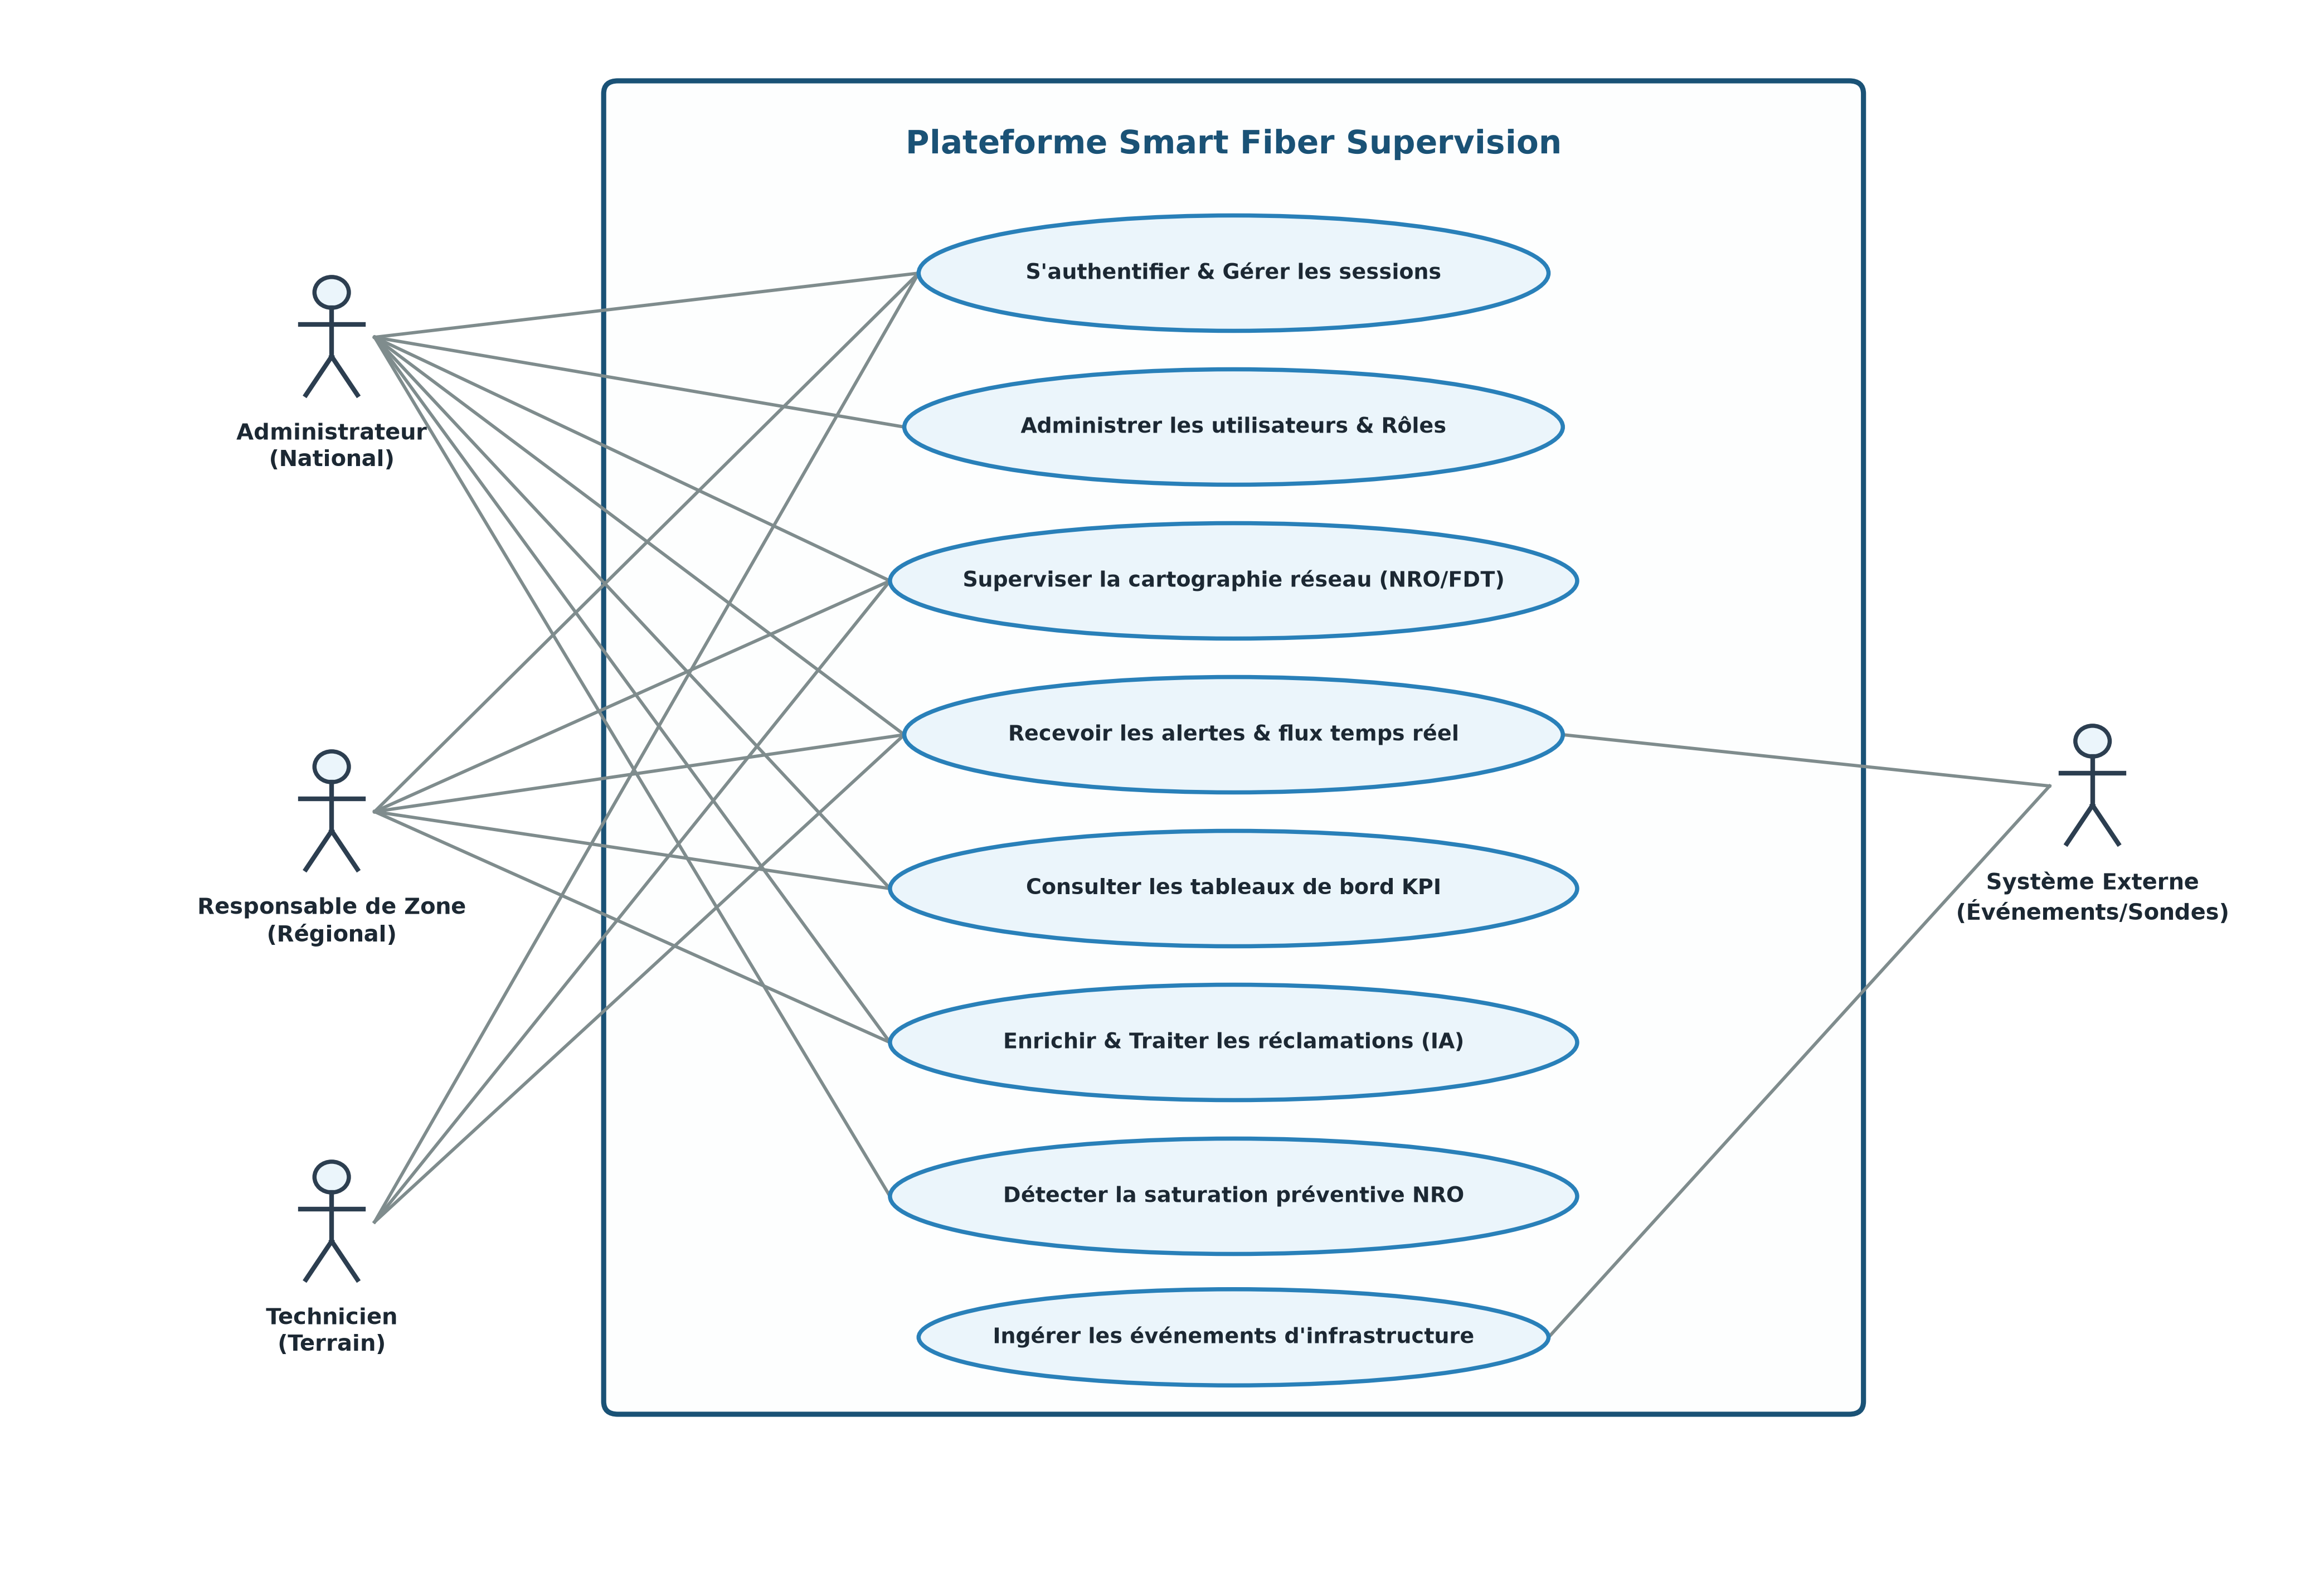
\includegraphics[width=15cm]{Images/usecase_global.png}
 \caption{Diagramme de cas d'utilisation global du syst\`eme}
 \label{fig:usecase-global}
\end{figure}

\subsection{Mod\`ele conceptuel de donn\'ees (Diagramme de classes global)}
La mod\'elisation conceptuelle du domaine t\'el\'ecom est illustr\'ee par la figure~\ref{fig:class-global}. Elle structure les relations entre les utilisateurs, les p\'erim\`etres g\'eographiques (\textit{Zone}), les \'equipements physiques optiques (\textit{NRO}, \textit{FDT}), les contrats abonn\'es et les r\'eclamations.

\begin{figure}[H]
 \centering
 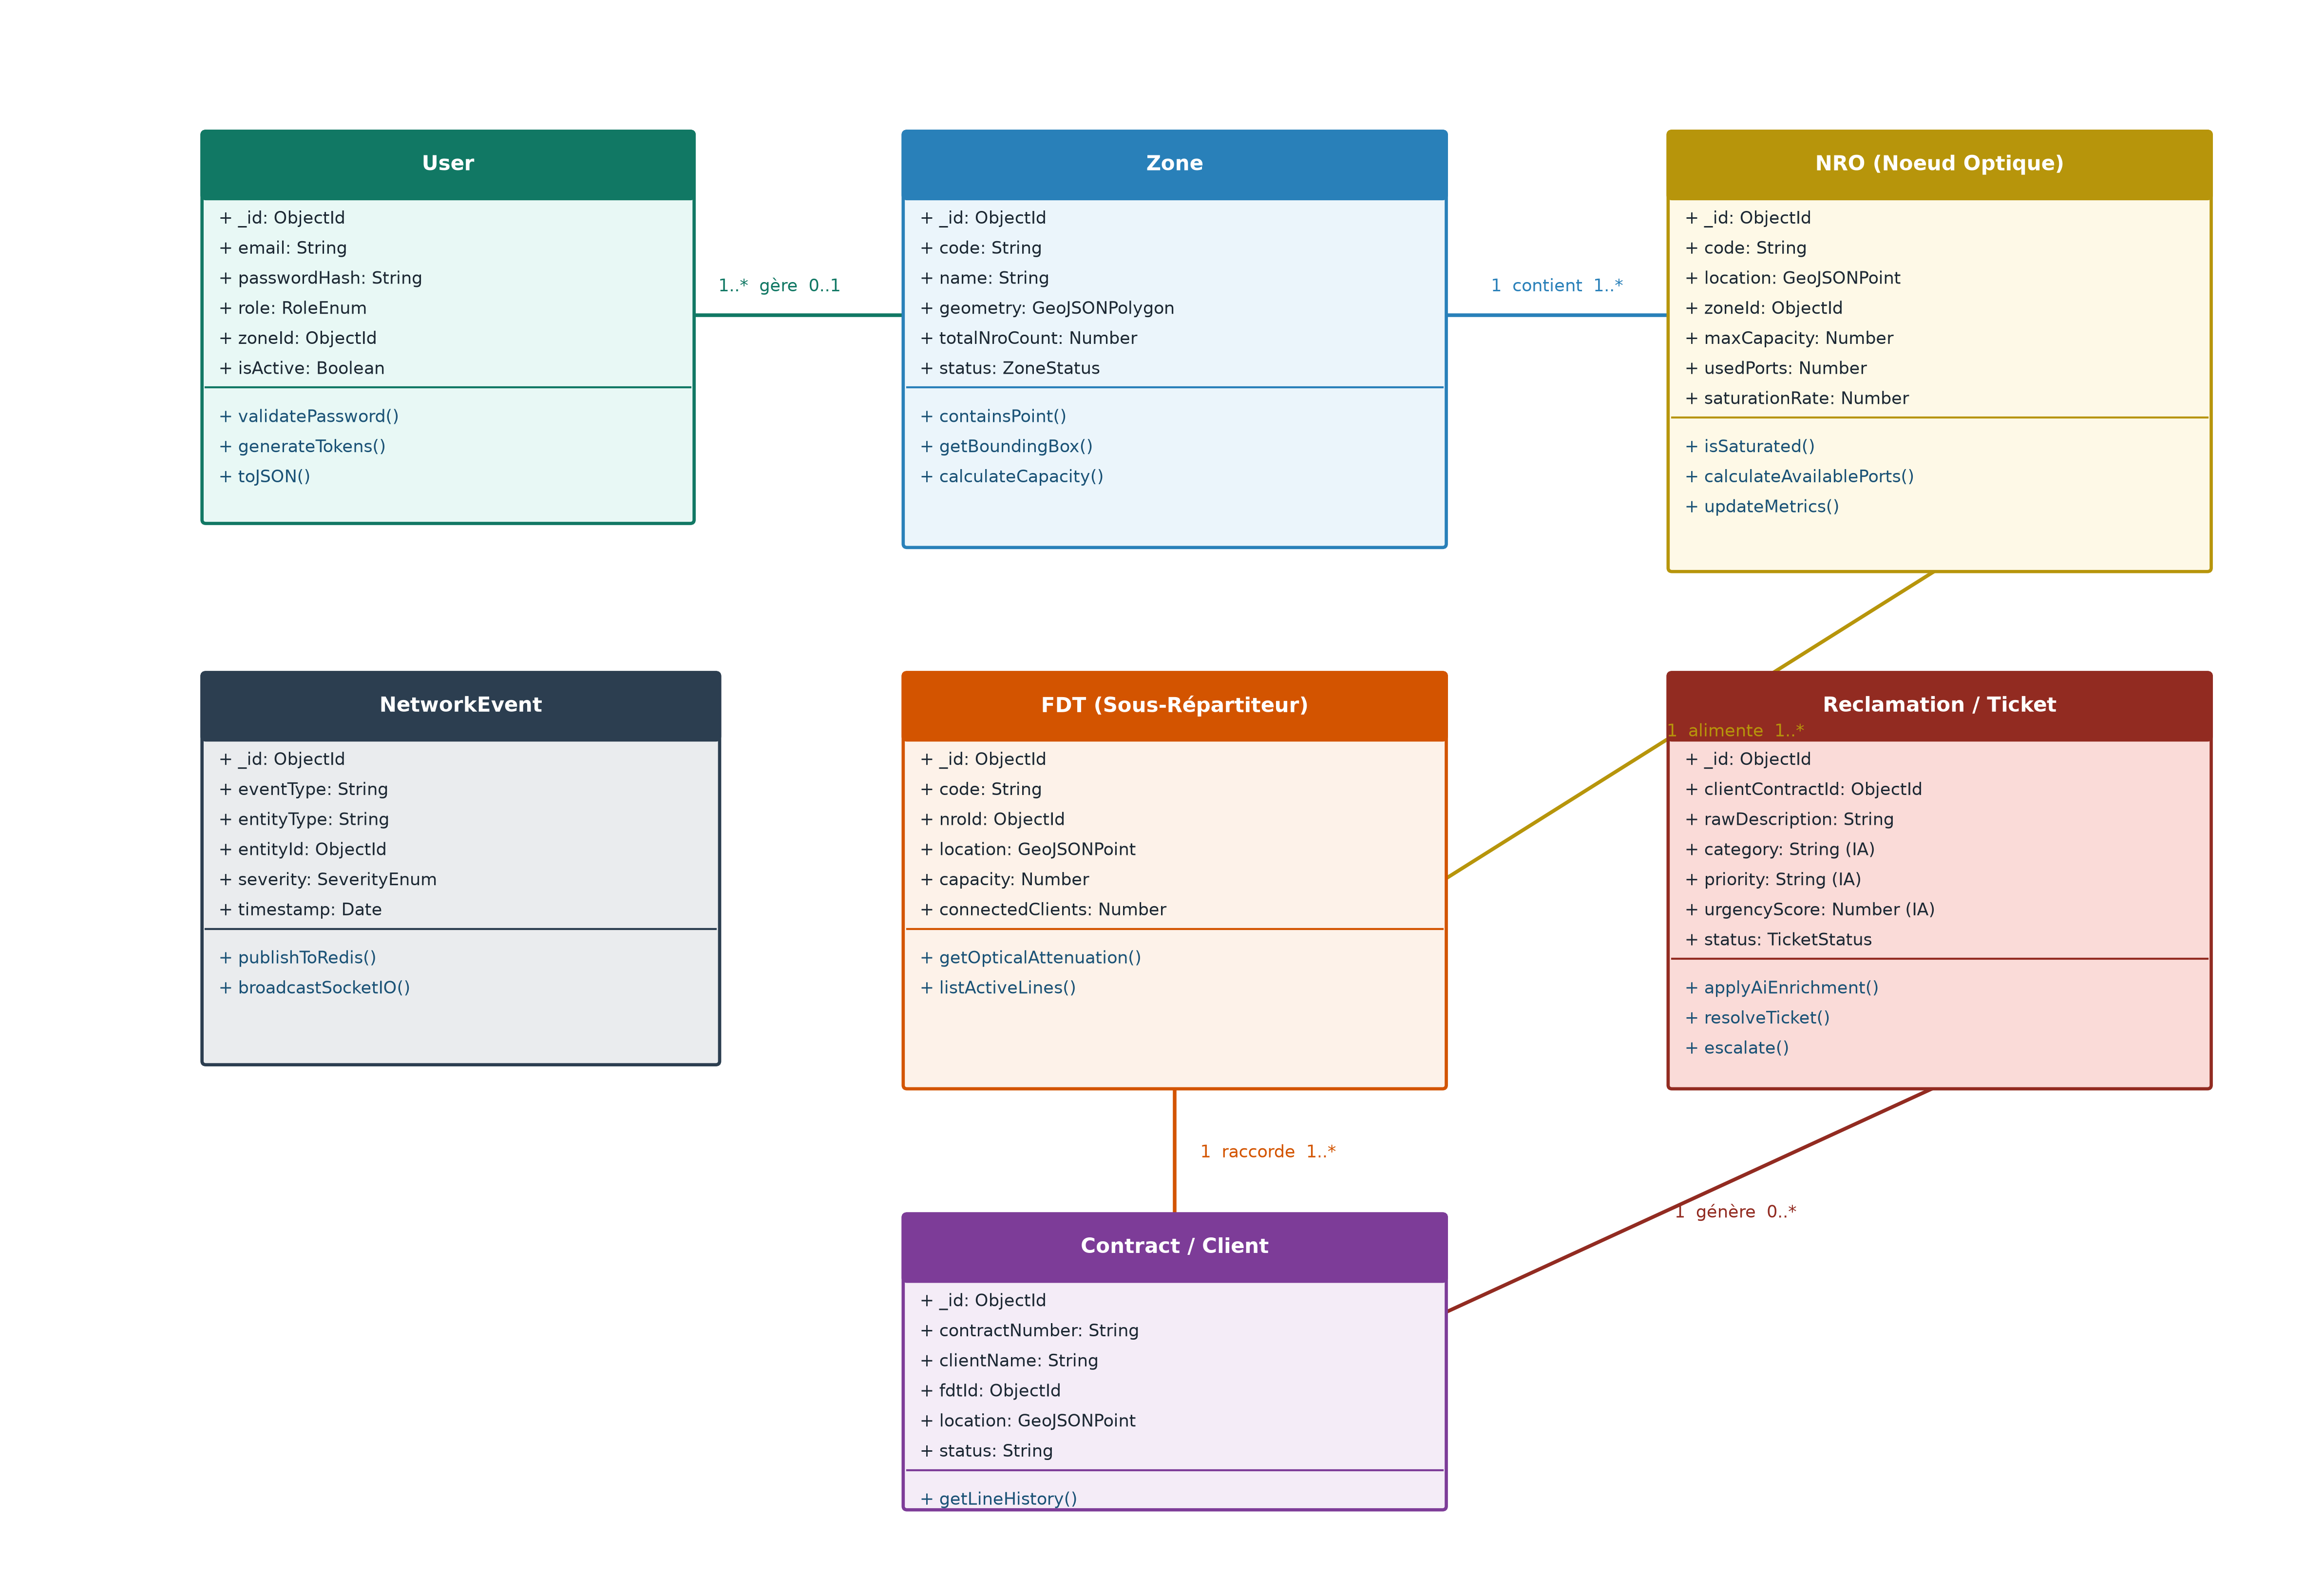
\includegraphics[width=15cm]{Images/class_global.png}
 \caption{Diagramme de classes conceptuel global du domaine m\'etier}
 \label{fig:class-global}
\end{figure}

\subsection{Vue d'ensemble de l'architecture fonctionnelle}
L'\'ecosyst\`eme logiciel s'articule autour de trois flux directeurs :
\begin{itemize}
    \item \textbf{Flux Administratif et Consultation (REST / HTTPS) :} Les requ\^etes de gestion CRUD et de chargement initial des couches cartographiques s'ex\'ecutent via l'API REST s\'ecuris\'ee par JWT.
    \item \textbf{Flux \'Ev\'enementiel et Alertes (WebSockets / WSS) :} Les changements d'\'etats r\'eseau et nouvelles r\'eclamations sont pouss\'es instantan\'ement vers l'application mobile.
    \item \textbf{Flux Asynchrone \& IA :} Les traitements lourds (analyse s\'emantique LLM, \'evaluation de la capacit\'e des NRO) sont d\'ecoupl\'es via les files BullMQ afin de garantir une disponibilit\'e maximale.
\end{itemize}

\section*{Conclusion}
Ce chapitre a permis de d\'efinir rigoureusement les besoins fonctionnels et non fonctionnels, d'identifier les r\^oles des acteurs et de structurer le backlog Scrum du projet. La conception globale a \'etabli les mod\`eles conceptuels de r\'ef\'erence. Les trois chapitres suivants pr\'esentent en d\'etail la r\'ealisation technique des trois releases du projet.     % Chapitre 2 : Analyse des besoins et conception générale
\include{chapters/sprint_socle}     % Chapitre 3 : Release 1 : Socle technique, Authentification et Gestion des Utilisateurs
\include{chapters/sprint_superv}    % Chapitre 4 : Release 2 : Supervision réseau, Cartographie et Temps réel
\include{chapters/sprint_ia_deploy} % Chapitre 5 : Release 3 : IA métier, Tests, Déploiement et Industrialisation
\chapter*{Conclusion g\'en\'erale et Perspectives}
\addcontentsline{toc}{chapter}{Conclusion g\'en\'erale et Perspectives}

\section*{Bilan des r\'ealisations}
Ce projet de fin d'\'etudes, men\'e en collaboration avec \textbf{Tunisie Telecom}, s'est donn\'e pour ambition de concevoir et r\'ealiser une plateforme compl\`ete et unifi\'ee de supervision r\'eseau fibre optique (FTTH), combinant r\'eactivit\'e temps r\'eel, cartographie interactive et aide \`a la d\'ecision bas\'ee sur l'intelligence artificielle.

L'ensemble des objectifs fix\'es au d\'epart a \'et\'e atteint avec succ\`es \`a travers trois releases incr\'ementales :
\begin{itemize}
    \item \textbf{Socle architectural et s\'ecurit\'e :} Mise en place d'une architecture client-serveur d\'ecoupl\'ee et robuste, s\'ecuris\'ee par JWT/RBAC et int\'egrant une gouvernance fine des acc\`es par zone g\'eographique.
    \item \textbf{Supervision cartographique et temps r\'eel :} D\'eveloppement d'une application mobile en Flutter int\'egrant une carte g\'eographique interactive multi-couches (NRO, FDT, clients, pannes) synchronis\'ee instantan\'ement via des WebSockets (Socket.IO).
    \item \textbf{Intelligence artificielle et r\'esilience :} Int\'egration r\'eussie du superviseur IA via Groq LLM pour l'enrichissement s\'emantique automatique des r\'eclamations et la d\'etection pr\'eventive de la saturation des NRO, appuy\'e par un patron de r\'esilience \textit{Circuit Breaker} avec repli heuristique.
\end{itemize}

\section*{D\'efis techniques surmont\'es}
Durant les diff\'erentes phases du cycle de d\'eveloppement, plusieurs d\'efis techniques majeurs ont \'et\'e relev\'es :
\begin{itemize}
    \item \textbf{Performance du rendu cartographique mobile :} L'affichage fluide de nombreuses entit\'es g\'eom\'etriques a n\'ecessit\'e une indexation spatiale optimis\'ee sous MongoDB (\textit{2dsphere}) et des m\'ecanismes de filtrage par zone visible (\textit{Bounding Box}).
    \item \textbf{R\'econciliation temps r\'eel :} La synchronisation transparente entre les \'ev\'enements serveur pouss\'es par WebSockets et l'\'etat applicatif local Flutter a \'et\'e r\'esolue efficacement gr\^ace \`a \textbf{Riverpod}.
    \item \textbf{Tol\'erance aux pannes et gestion des quotas IA :} La mise en \oe uvre du Circuit Breaker garantit une continuit\'e totale de service m\^eme en cas d'indisponibilit\'e des services tiers.
\end{itemize}

\section*{Apports personnels et professionnels}
Sur le plan personnel et technique, ce projet a constitu\'e une exp\'erience tr\`es enrichissante. Il nous a permis d'approfondir nos comp\'etences dans le d\'eveloppement full-stack moderne (NestJS, Flutter), l'ing\'enierie des syst\`emes temps r\'eel et g\'eospatiaux, l'int\'egration de l'IA g\'en\'erative en milieu d'entreprise, ainsi que l'application rigoureuse des pratiques d'ing\'enierie logicielle et de la m\'ethodologie Agile Scrum.

\section*{Perspectives d'\'evolution}
Pour prolonger les r\'esultats obtenus, plusieurs axes d'am\'elioration et perspectives futures peuvent \^etre envisag\'es :
\begin{enumerate}
    \item \textbf{Mode hors-ligne pour techniciens terrain :} Int\'egrer une base de donn\'ees locale embarqu\'ee (ex : Isar / SQLite) avec synchronisation diff\'er\'ee bidirectionnelle afin de permettre l'utilisation de l'application mobile m\^eme dans les sous-sols et zones d\'epourvues de couverture 4G/5G.
    \item \textbf{Mod\`eles pr\'edictifs avanc\'es :} Entra\^iner des mod\`eles d'apprentissage automatique d\'edi\'es (\textit{Machine Learning / Time Series}) sur l'historique des pannes afin de pr\'edire les d\'efaillances d'\'equipements avant leur survenue.
    \item \textbf{Interop\'erabilit\'e SIG avanc\'ee :} \'Etendre les capacit\'es d'import/export de fichiers cartographiques standardis\'es (Shapefile, GeoJSON, KML) pour une int\'egration directe avec les outils SIG d'entreprise comme QGIS ou ArcGIS.
\end{enumerate}
       % Conclusion générale et Perspectives
\chapter*{Netographie}
\addcontentsline{toc}{chapter}{Netographie}

Cette section regroupe les sources web, la documentation technique et les r\'ef\'erences utilis\'ees pour r\'ediger le rapport.

\begin{itemize}
	\item Documentation Flutter : \url{https://docs.flutter.dev/}
	\item Documentation NestJS : \url{https://docs.nestjs.com/}
	\item Documentation Riverpod : \url{https://riverpod.dev/}
	\item Documentation Socket.IO : \url{https://socket.io/docs/v4/}
\end{itemize}
      % Netographie

\end{document}
